% !TEX TS-program = pdflatex
\documentclass[11pt]{article}

% -------------------- Packages --------------------
\usepackage[a4paper,margin=1in]{geometry}
\usepackage{amsmath,amssymb}
\usepackage[T1]{fontenc}
\usepackage{lmodern}
\usepackage{xcolor}
\usepackage{tcolorbox}
\tcbuselibrary{skins,breakable}
\usepackage{enumitem}
\usepackage{hyperref}
\usepackage{tikz}
\usetikzlibrary{calc,arrows.meta,angles,quotes}

\pagestyle{empty}

% -------------------- Dark Theme Colors --------------------
\definecolor{bg}{HTML}{000000}
\definecolor{pairbg}{HTML}{121212}
\definecolor{solbg}{HTML}{0A0A0A}
\definecolor{border}{HTML}{2A2A2A}
\definecolor{text}{HTML}{FFFFFF}
\definecolor{muted}{HTML}{C9CDD3}
\definecolor{gold}{HTML}{FFD700}
\definecolor{green}{HTML}{4ADE80}
\definecolor{cyan}{HTML}{38BDF8}

\pagecolor{bg}
\color{text}

\hypersetup{
  colorlinks=true,
  linkcolor=cyan,
  urlcolor=cyan
}

\setlength{\parindent}{0pt}
\setlength{\parskip}{10pt}

\setlist[itemize]{left=1.4em,itemsep=6pt,topsep=6pt}
\setlist[enumerate]{left=1.6em,itemsep=4pt,topsep=4pt}

% -------------------- tcolorbox Base --------------------
\tcbset{
  enhanced,
  breakable,
  arc=12pt,
  boxrule=0.8pt,
  left=16pt,right=16pt,top=12pt,bottom=12pt
}

\newtcolorbox{QAPair}[1]{%
  colback=pairbg,
  colbacklower=solbg,
  colframe=border,
  coltext=text,
  title=\textcolor{gold}{\bfseries #1},
  fonttitle=\bfseries,
  coltitle=text,
  segmentation style={draw=border, dashed, line width=0.6pt},
}

\newtcolorbox{QuickBox}{%
  colback=pairbg,
  colframe=cyan,
  coltext=text,
  fontupper=\color{text},
  borderline north={4pt}{0pt}{cyan},
  arc=14pt,
  boxrule=0.8pt
}

\newcommand{\Step}[1]{\textcolor{muted}{\textbf{Step #1:}}}

% -------------------- TikZ Styles --------------------
\tikzset{
  axis/.style={->, draw=muted, line width=0.8pt},
  route/.style={->, draw=cyan, line width=1.1pt},
  edge/.style={draw=cyan, line width=1.1pt},
  dashedhelp/.style={draw=muted, dashed, line width=0.8pt},
  pt/.style={circle, fill=gold, inner sep=1.5pt},
  lab/.style={text=text, font=\small},
  note/.style={text=muted, font=\small}
}

% ============================================================
\begin{document}

\begin{center}
{\LARGE\bfseries \textcolor{gold}{Exercise 6.6 --- Solutions}}\\[-2pt]
\end{center}

\begin{QuickBox}
{\color{cyan}\bfseries Quick formulas (bearings)}\par\medskip
\begin{itemize}
\item \textbf{Reverse bearing:} if $\theta<180^\circ$ then $\theta+180^\circ$; if $\theta\ge 180^\circ$ then $\theta-180^\circ$.
\item \textbf{Components (distance $d$, bearing $\theta$):} East $=d\sin\theta$, North $=d\cos\theta$.
\item \textbf{Distance from components:} $d=\sqrt{E^2+N^2}$.
\item \textbf{Right angle check:} angle between two bearings is the (small) difference of the bearings.
\end{itemize}
\end{QuickBox}

% ============================================================
\begin{QAPair}{Question 3}
\textcolor{gold}{\bfseries Question:} Two boats $A$ and $B$ are $5$ km apart and the bearing of $B$ from $A$ is $250^\circ$. Draw the diagram showing relative positions, then find the bearing of $A$ from $B$.\par
\tcblower
\textcolor{green}{\bfseries Answer:}
\[
\begin{aligned}
\Step{1}\;& \text{Bearing of }B\text{ from }A = 250^\circ.\\
\Step{2}\;& \text{Reverse bearing (from }B\text{ to }A):\ 250^\circ-180^\circ=70^\circ.\\
\Step{3}\;& \Rightarrow\ \text{bearing of }A\text{ from }B = \boxed{070^\circ}.
\end{aligned}
\]

\textcolor{muted}{\bfseries Sketch:}\par
\begin{center}
\begin{tikzpicture}[scale=1.0]
  \coordinate (A) at (0,0);
  % bearing 250 -> tikz angle = 90-250=-160 = 200
  \coordinate (B) at ($(A)+(200:3.3)$);

  \draw[axis] (A) -- ++(0,2.3) node[lab, above] {N};
  \draw[axis] (A) -- ++(2.4,0) node[lab, right] {E};

  \draw[route] (A) -- (B) node[midway, note, below] {$5$ km};

  \node[pt,label={[lab]below left:$A$}] at (A) {};
  \node[pt,label={[lab]below:$B$}] at (B) {};

  % small bearing cue from north at A
  \draw[dashedhelp] (A) ++(0,1.6) arc[start angle=90,end angle=-70,radius=1.6];
  \node[note] at ($(A)+(0.9,1.35)$) {$250^\circ$};

  \node[note] at ($(B)+(-1.2,1.0)$) {Reverse: $070^\circ$};
\end{tikzpicture}
\end{center}
\end{QAPair}

% ============================================================
\begin{QAPair}{Question 4}
\textcolor{gold}{\bfseries Question:} The positions of three ships $A,B,C$ are such that the bearing of $B$ from $A$ is $045^\circ$ and ship $C$ is to the east of $A$. If bearing of $C$ from $B$ is $180^\circ$ and $AB=10$ km, what is the bearing of $A$ from $C$? Also find the distance between ship $A$ and ship $C$.\par
\tcblower
\textcolor{green}{\bfseries Answer:}
\[
\begin{aligned}
\Step{1}\;& AB=10,\ \text{bearing }A\to B=45^\circ\\
&\Rightarrow \text{East component}=10\sin45^\circ=5\sqrt2,\ \text{North component}=10\cos45^\circ=5\sqrt2.\\
\Step{2}\;& \text{Bearing }B\to C=180^\circ \Rightarrow C \text{ is due south of }B.\\
\Step{3}\;& C \text{ is due east of }A \Rightarrow C \text{ has same northing as }A \ (0).\\
\Step{4}\;& \text{So drop }B \text{ down to northing }0:\ BC=5\sqrt2\ \text{km}.\\
\Step{5}\;& \Rightarrow C=(5\sqrt2,0)\ \text{and}\ AC=5\sqrt2\ \text{km}\approx 7.07\ \text{km}.\\
\Step{6}\;& \text{From }C\text{ to }A\text{ is due west} \Rightarrow \text{bearing }C\to A=\boxed{270^\circ}.
\end{aligned}
\]
\[
\boxed{AC=5\sqrt2\ \text{km}\approx 7.07\ \text{km},\qquad \text{bearing of }A\text{ from }C=270^\circ.}
\]

\textcolor{muted}{\bfseries Sketch:}\par
\begin{center}
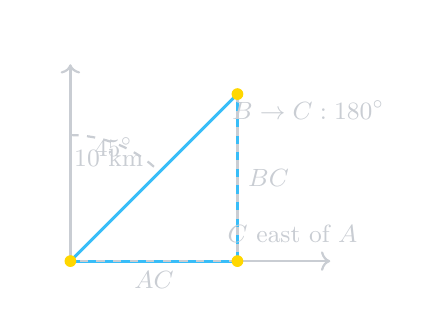
\begin{tikzpicture}[scale=1.0]
  \coordinate (A) at (0,0);
  % bearing 45 => tikz angle 90-45=45
  \coordinate (B) at ($(A)+(45:3.0)$);
  % C is east of A and due south of B => same x as B, y=0
  \coordinate (C) at ($(B|-A)$);

  \draw[axis] (A) -- ++(0,2.5) node[lab, above] {N};
  \draw[axis] (A) -- ++(3.3,0) node[lab, right] {E};

  \draw[edge] (A) -- (B) node[midway, note, above left] {$10$ km};
  \draw[edge] (B) -- (C) node[midway, note, right] {$BC$};
  \draw[edge] (A) -- (C) node[midway, note, below] {$AC$};

  \draw[dashedhelp] (B) -- ($(B|-A)$);
  \draw[dashedhelp] (C) -- (A);

  \node[pt,label={[lab]below left:$A$}] at (A) {};
  \node[pt,label={[lab]above:$B$}] at (B) {};
  \node[pt,label={[lab]below:$C$}] at (C) {};

  % bearing cue at A
  \draw[dashedhelp] (A) ++(0,1.6) arc[start angle=90,end angle=45,radius=1.6];
  \node[note] at ($(A)+(0.55,1.45)$) {$45^\circ$};

  \node[note] at ($(B)+(0.9,-0.2)$) {$B\to C:180^\circ$};
  \node[note] at ($(C)+(0.7,0.35)$) {$C$ east of $A$};
\end{tikzpicture}
\end{center}
\end{QAPair}

% ============================================================
\begin{QAPair}{Question 5}
\textcolor{gold}{\bfseries Question:} Babar walked from point $P$ to point $Q$ at a bearing of $050^\circ$ for $3$ km. Then he walked from $Q$ to $R$ at a bearing of $140^\circ$. Find the distance $QR$, if the distance between $P$ and $R$ is $5$ km. Also find the bearing of $R$ from $P$.\par
\tcblower
\textcolor{green}{\bfseries Answer:}

\textcolor{muted}{\bfseries Part A: Find $QR$}\par
\[
\begin{aligned}
\Step{1}\;& \text{Bearing }P\to Q=50^\circ \Rightarrow \text{bearing }Q\to P=50^\circ+180^\circ=230^\circ.\\
\Step{2}\;& \text{Bearing }Q\to R=140^\circ.\\
\Step{3}\;& \angle PQR=\bigl|230^\circ-140^\circ\bigr|=90^\circ \Rightarrow \triangle PQR \text{ right-angled at }Q.\\
\Step{4}\;& PR^2=PQ^2+QR^2 \Rightarrow 5^2=3^2+QR^2 \Rightarrow QR^2=16 \Rightarrow \boxed{QR=4\text{ km}}.
\end{aligned}
\]

\textcolor{muted}{\bfseries Part B: Bearing of $R$ from $P$}\par
Use components (East $=d\sin\theta$, North $=d\cos\theta$):
\[
\begin{aligned}
E_{PR}&=3\sin50^\circ+4\sin140^\circ,\\
N_{PR}&=3\cos50^\circ+4\cos140^\circ.
\end{aligned}
\]
Numerically,
\[
E_{PR}\approx 4.869,\qquad N_{PR}\approx -1.136.
\]
So $R$ lies \textbf{south-east} of $P$. Angle east of south is
\[
\alpha=\tan^{-1}\!\left(\frac{E_{PR}}{|N_{PR}|}\right)\approx 76.87^\circ.
\]
Hence bearing from north:
\[
\theta=180^\circ-\alpha\approx 103.13^\circ\approx \boxed{103^\circ}.
\]

\[
\boxed{QR=4\text{ km},\qquad \text{bearing of }R\text{ from }P\approx 103^\circ.}
\]

\textcolor{muted}{\bfseries Sketch:}\par
\begin{center}
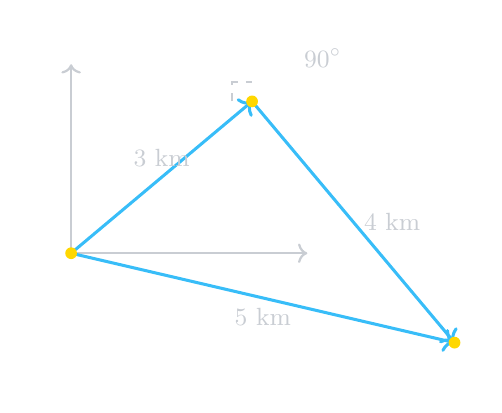
\begin{tikzpicture}[scale=1.0]
  \coordinate (P) at (0,0);
  \coordinate (Q) at ($(P)+(40:3)$);   % bearing 50 -> tikz angle 40
  \coordinate (R) at ($(Q)+(-50:4)$);  % bearing 140 -> tikz angle -50
  \draw[axis] (P) -- ++(0,2.4) node[lab, above] {N};
  \draw[axis] (P) -- ++(3.0,0) node[lab, right] {E};

  \draw[route] (P) -- (Q) node[midway, note, above] {$3$ km};
  \draw[route] (Q) -- (R) node[midway, note, right] {$4$ km};
  \draw[route] (P) -- (R) node[midway, note, below] {$5$ km};

  \node[pt,label={[lab]below left:$P$}] at (P) {};
  \node[pt,label={[lab]above:$Q$}] at (Q) {};
  \node[pt,label={[lab]below:$R$}] at (R) {};

  \draw[dashedhelp] ($(Q)+(-0.25,0)$) -- ++(0,0.25) -- ++(0.25,0);
  \node[note] at ($(Q)+(0.9,0.55)$) {$90^\circ$};
\end{tikzpicture}
\end{center}
\end{QAPair}

% ============================================================
\begin{QAPair}{Question 6}
\textcolor{gold}{\bfseries Question:} Rayyan spots a snake directly north from his location. Sarim is $25$m east of Rayyan and spots the same snake. If the bearing of Sarim from the snake is $122^\circ$, how far is Rayyan from the snake?\par
\tcblower
\textcolor{green}{\bfseries Answer:}
Let Rayyan be at $(0,0)$, Sarim at $(25,0)$ and snake at $(0,d)$.

\[
\begin{aligned}
\Step{1}\;& \overrightarrow{\text{snake}\to \text{Sarim}}=(25,\,-d).\\
\Step{2}\;& \text{Bearing }=122^\circ \Rightarrow
\frac{\text{East}}{\text{North}}=\tan 122^\circ
\Rightarrow \frac{25}{-d}=\tan 122^\circ.\\
\Step{3}\;& d=-\frac{25}{\tan 122^\circ}\approx 15.62.
\end{aligned}
\]
\[
\boxed{\text{Rayyan is about }15.6\text{ m from the snake.}}
\]

\textcolor{muted}{\bfseries Sketch (not to scale):}\par
\begin{center}
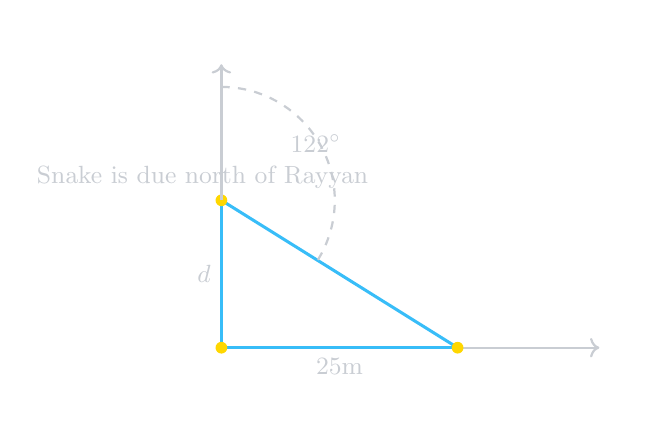
\begin{tikzpicture}[scale=0.12]
  % scaled: 1 unit = 1 m (scale makes it fit)
  \coordinate (R) at (0,0);      % Rayyan
  \coordinate (Sa) at (25,0);    % Sarim (25 m east)
  \coordinate (Sn) at (0,15.6);  % Snake (approx d north)

  % axes at Rayyan
  \draw[axis] (R) -- ++(0,30) node[lab, above] {N};
  \draw[axis] (R) -- ++(40,0) node[lab, right] {E};

  % triangle
  \draw[edge] (R) -- (Sn) node[midway, note, left] {$d$};
  \draw[edge] (R) -- (Sa) node[midway, note, below] {$25$m};
  \draw[edge] (Sn) -- (Sa);

  \node[pt,label={[lab]below left:Rayyan}] at (R) {};
  \node[pt,label={[lab]below: Sarim}] at (Sa) {};
  \node[pt,label={[lab]above left:Snake}] at (Sn) {};

  % bearing arc at Snake: from north (up) clockwise to line Sn->Sa
  \draw[dashedhelp] (Sn) -- ++(0,12);
  \draw[dashedhelp] (Sn) ++(0,12) arc[start angle=90, end angle=-32, radius=12];
  \node[note] at ($(Sn)+(10,6)$) {$122^\circ$};

  % right-angle cue of "snake directly north of Rayyan"
  \node[note] at ($(R)+(-2,18)$) {Snake is due north of Rayyan};
\end{tikzpicture}
\end{center}
\end{QAPair}

% ============================================================
\begin{QAPair}{Question 7}
\textcolor{gold}{\bfseries Question:} Bilal traveled $12$ km to reach school at a bearing of $060^\circ$ from his home. Then he went to the football ground from school at a bearing of $150^\circ$. If the football ground is $5$ km from school, find the distance from the football ground to his home.\par
\tcblower
\textcolor{green}{\bfseries Answer:}
\[
\begin{aligned}
\Step{1}\;& \text{Bearing home}\to\text{school}=60^\circ \Rightarrow \text{school}\to\text{home}=240^\circ.\\
\Step{2}\;& \text{Bearing school}\to\text{ground}=150^\circ.\\
\Step{3}\;& \angle(\text{home from school},\ \text{ground from school})
=|240^\circ-150^\circ|=90^\circ.\\
\Step{4}\;& \triangle \text{(home, school, ground)}\ \text{is right-angled at school}.\\
\Step{5}\;& \text{Distance (ground to home)}=\sqrt{12^2+5^2}=\sqrt{169}= \boxed{13\text{ km}}.
\end{aligned}
\]

\textcolor{muted}{\bfseries Sketch:}\par
\begin{center}
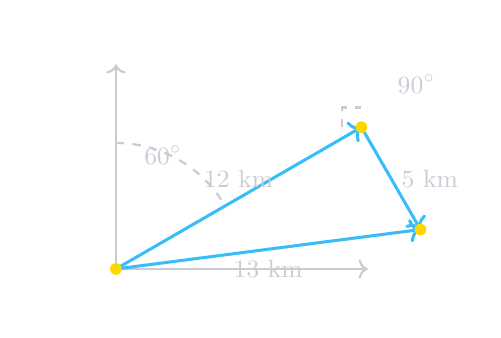
\begin{tikzpicture}[scale=1.0]
  \coordinate (H) at (0,0);                 % Home
  \coordinate (S) at ($(H)+(30:3.6)$);      % bearing 60 -> tikz 30, scaled length
  \coordinate (G) at ($(S)+(-60:1.5)$);     % bearing 150 -> tikz -60, scaled

  \draw[axis] (H) -- ++(0,2.6) node[lab, above] {N};
  \draw[axis] (H) -- ++(3.2,0) node[lab, right] {E};

  \draw[route] (H) -- (S) node[midway, note, above] {$12$ km};
  \draw[route] (S) -- (G) node[midway, note, right] {$5$ km};
  \draw[route] (H) -- (G) node[midway, note, below] {$13$ km};

  \node[pt,label={[lab]below left:Home}] at (H) {};
  \node[pt,label={[lab]above:School}] at (S) {};
  \node[pt,label={[lab]below:Ground}] at (G) {};

  % right angle marker at S
  \draw[dashedhelp] ($(S)+(-0.25,0)$) -- ++(0,0.25) -- ++(0.25,0);
  \node[note] at ($(S)+(0.7,0.55)$) {$90^\circ$};

  % small bearing cue at H for 60
  \draw[dashedhelp] (H) ++(0,1.6) arc[start angle=90,end angle=30,radius=1.6];
  \node[note] at ($(H)+(0.6,1.45)$) {$60^\circ$};
\end{tikzpicture}
\end{center}
\end{QAPair}

% ============================================================
\begin{QAPair}{Question 8}
\textcolor{gold}{\bfseries Question:} A car leaves the garage at a bearing of $040^\circ$ and travels in a straight line for $13$ km. How many kilometres north and how many kilometres east has the car traveled?\par
\tcblower
\textcolor{green}{\bfseries Answer:}
\[
\begin{aligned}
\Step{1}\;& \text{North} = 13\cos 40^\circ \approx 13(0.7660)=9.96\text{ km}.\\
\Step{2}\;& \text{East}  = 13\sin 40^\circ \approx 13(0.6428)=8.36\text{ km}.
\end{aligned}
\]
\[
\boxed{\text{North }\approx 9.96\text{ km},\qquad \text{East }\approx 8.36\text{ km}.}
\]

\textcolor{muted}{\bfseries Sketch (components):}\par
\begin{center}
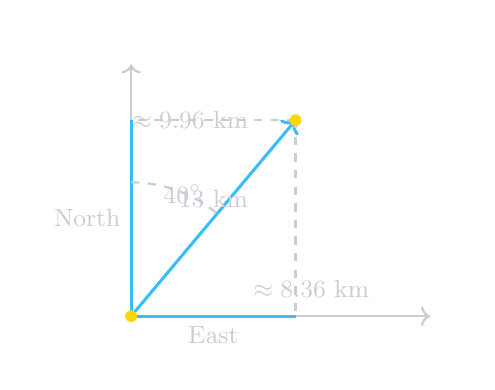
\begin{tikzpicture}[scale=1.0]
  \coordinate (G) at (0,0);                 % Garage
  \coordinate (P) at ($(G)+(50:3.25)$);     % bearing 40 -> tikz 50, scaled (13 km)
  \coordinate (Eproj) at ($(P|-G)$);        % drop to east-axis
  \coordinate (Nproj) at ($(G|-P)$);        % up the north-axis

  \draw[axis] (G) -- ++(0,3.2) node[lab, above] {N};
  \draw[axis] (G) -- ++(3.8,0) node[lab, right] {E};

  \draw[route] (G) -- (P) node[midway, note, above] {$13$ km};

  % projections
  \draw[dashedhelp] (P) -- (Eproj);
  \draw[dashedhelp] (P) -- (Nproj);

  \draw[edge] (G) -- (Eproj) node[midway, note, below] {East};
  \draw[edge] (G) -- (Nproj) node[midway, note, left] {North};

  \node[pt,label={[lab]below left:Garage}] at (G) {};
  \node[pt,label={[lab]above:Car}] at (P) {};

  % bearing arc at G (40 degrees clockwise from north)
  \draw[dashedhelp] (G) ++(0,1.7) arc[start angle=90,end angle=50,radius=1.7];
  \node[note] at ($(G)+(0.65,1.55)$) {$40^\circ$};

  \node[note] at ($(Eproj)+(0.2,0.35)$) {$\approx 8.36$ km};
  \node[note] at ($(Nproj)+(0.75,0.0)$) {$\approx 9.96$ km};
\end{tikzpicture}
\end{center}
\end{QAPair}

\end{document}
